\chapter{密度与换测度}
\label{chap:densities-change-of-measure}

同一个可测空间上常常同时出现两种测度。抛一枚不均匀的骰子，可以拿“每个点数算一份”的计数作参考，也可以拿另一枚骰子的概率作参考；描述实轴上的随机误差，参考对象通常是长度。第~\ref{chap:measures}章已经比较过这样两种测度：绝对连续说明一种测度忽略的集合另一种也忽略，Lebesgue分解把目标测度拆成参考测度能够“看见”的部分和集中在参考零测集上的部分。这些关系都只涉及集合的质量，还没有回答一个更具体的问题：能否用一个逐点的权重函数，把参考测度的质量换算成目标测度的质量？

第~\ref{chap:integration}章建立积分以后，这个问题就有了准确的说法。若非负可测函数$h$对每个可测集$A$都满足$\nu(A)=\int_Ah\,\mathrm d\mu$，$h$就是$\nu$相对于$\mu$的密度。本章围绕三个问题展开：密度是什么、何时存在、怎样计算和使用。读完本章，读者应能判断给定的两个测度之间是否存在密度，在$\sigma$有限的条件下证明它的存在与几乎处处唯一，用它在两种测度之间转换积分，并对离散质量、函数增量和映射后的质量写出具体的密度。

路线如下。第~\ref{sec:density-relative}节从有限点集上的质量之比出发定义密度，并说明给定权重总能产生一个测度、改动参考零测集上的取值不影响结果。第~\ref{sec:density-existence}节反过来从两个已知测度寻找密度，证明Radon–Nikodym定理，并把它接到Lebesgue分解与有符号测度上。第~\ref{sec:density-rules}节研究有了密度之后怎样换参考测度：换测度公式、线性组合、链式规则与倒数。第~\ref{sec:density-computation}节把这些结论落实到离散测度、由函数增量产生的测度和推前测度上。积分的定义、单调收敛与控制收敛直接引用第~\ref{chap:integration}章，不在这里重复。

\section{相对密度}
\label{sec:density-relative}

本节固定同一可测空间$(X,\mathcal A)$上的两个非负测度：一个充当参考，一个是要描述的目标。先在有限点集上看清“密度就是质量之比”，再借助第~\ref{chap:integration}章的积分把这个想法推广到一般测度。随后从相反的方向说明：任给参考测度和非负权重，积分总能产生一个新测度；最后说明密度只在参考测度的几乎处处意义下有意义。

\subsection{参考测度与密度的定义}
\label{sec:density-definition}

\paragraph{有限点集上的质量之比}
设$X=\{a,b,c\}$，目标测度$\nu$给三个点的质量分别为$0.2,0.5,0.3$。若参考测度是计数测度，每点质量为$1$，那么要从参考质量得到目标质量，只需在每点乘以$0.2,0.5,0.3$。若参考测度改为$\mu'=2\delta_a+\delta_b+\delta_c$，点$a$的参考质量是$2$，乘数就要改成$0.2/2=0.1$，另外两点的乘数不变。一般地，参考测度在点$x_i$上的质量为$m_i>0$、目标质量为$p_i$时，该点的乘数是$p_i/m_i$；任一子集的目标质量都等于参考质量乘以乘数后求和，例如$\nu(\{a,b\})=0.1\cdot2+0.5\cdot1=0.7$。

图~\ref{fig:density-mass-ratio}并排画出这两种参考。读者应注意，目标测度在两栏中完全相同，变化的只有虚线框表示的参考质量，因而乘数$h$随之改变。密度描述的是“目标相对于参考”的换算比例，离开参考测度谈密度没有意义。

\begin{figure}[!htbp]
  \centering
  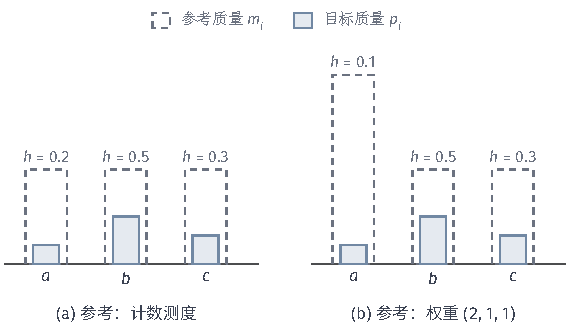
\includegraphics[width=96.651mm]{figures/02-abstract-mathematics/01-metric-and-measure/tikz/c4-mass-ratio/figure.pdf}
  \caption{密度是目标质量与参考质量之比。三点集$\{a,b,c\}$上的目标质量$p=(0.2,0.5,0.3)$（蓝色实心柱）保持不变。(a)参考为计数测度（虚线框高为$1$），每点的密度$h$等于目标质量本身；(b)参考权重改为$(2,1,1)$，点$a$的密度变为$0.2/2=0.1$，其余两点不变。}
  \label{fig:density-mass-ratio}
\end{figure}

\paragraph{一般测度上的密度}
有限点集上可以逐点做除法，是因为每一点都有正的参考质量。在实轴的长度测度下，每个单点的长度都是$0$，“单点质量相除”就成了$0/0$，所以一般情形不能逐点定义比值。可以保留的是另一半：在每个集合上，参考质量乘以权重再累计，应当得到目标质量。在有限点集上这个累计是求和，一般情形下就是第~\ref{chap:integration}章的积分。约定$\int_Ah\,\mathrm d\mu=\int_Xh\mathbf 1_A\,\mathrm d\mu$。

\begin{definition}[相对密度]
\label{def:density-density}
设$\mu,\nu$是可测空间$(X,\mathcal A)$上的非负测度。若可测函数$h:X\to[0,+\infty]$满足
\begin{equation}
 \nu(A)=\int_Ah\,\mathrm d\mu,\qquad A\in\mathcal A,
 \label{eq:density-definition}
\end{equation}
就称$h$是$\nu$相对于$\mu$的一个\term{相对密度}（relative density），也称\term{Radon–Nikodym密度}（Radon-Nikodym derivative），记作$\dfrac{\mathrm d\nu}{\mathrm d\mu}=h$；$\mu$称为\term{参考测度}（reference measure）。
\end{definition}

定义中说的是“一个”密度：后面会看到，在参考零测集上改动$h$不影响\eqref{eq:density-definition}，所以记号$\mathrm d\nu/\mathrm d\mu$只指其中任一个版本，含有它的等式都理解为$\mu$-几乎处处成立。这里没有新的积分理论，新增的只是用一个函数来表示两个测度之间的关系。记号$\mathrm d\nu/\mathrm d\mu$借用了导数的写法，但它不是对某个坐标求导，而是两种测度之间的换算权重。

\paragraph{概率质量函数与概率密度函数}
卷一用概率质量函数和概率密度函数描述随机变量的分布（可参考\BookChapterRef{chap:random-variables}{卷一“随机变量与概率分布”章}），二者都是上述定义的特例，区别只在参考测度。离散分布在可数集合$S$上的概率质量函数$p(s)$满足$\nu(A)=\sum_{s\in A}p(s)$；对计数测度$c$的积分就是求和（第~\ref{sec:integral-classical}节），所以$p$是$\nu$相对于$c$的密度。连续分布的概率密度函数$p$满足$\nu(A)=\int_Ap\,\mathrm d\lambda$，它是相对于Lebesgue测度$\lambda$的密度。

一般的密度不要求总积分为一：$\int_Xh\,\mathrm d\mu=\nu(X)$，只有目标测度是概率测度时这个值才是$1$。例如$[0,1]$上的$h(x)=2$是测度$2\lambda|_{[0,1]}$相对于$\lambda$的密度，总质量为$2$。另一方面，概率密度函数在某点的值可以大于$1$，因为它不是该点的概率；在长度测度下单点的概率总是$0$，密度值只有在集合上积分后才变成质量。

\subsection{由密度构造测度}
\label{sec:density-weighted-measure}

定义~\ref{def:density-density}是从两个已知测度出发的。反过来，若只给定参考测度和一个非负权重，按\eqref{eq:density-definition}的右边计算，是否总得到一个测度？答案是肯定的，而且不需要任何有限性条件。

\begin{theorem}[加权测度]
\label{thm:density-weighted-measure}
设$(X,\mathcal A,\mu)$是测度空间，$h:X\to[0,+\infty]$可测。令
\[
 \nu_h(A)=\int_Ah\,\mathrm d\mu,\qquad A\in\mathcal A .
\]
则$\nu_h$是$(X,\mathcal A)$上的非负测度，$h$是它相对于$\mu$的密度，并且$\nu_h\ll\mu$。
\end{theorem}

\begin{proof}
$\nu_h(\varnothing)=\int_X0\,\mathrm d\mu=0$，且$\nu_h$取值于$[0,+\infty]$。设$A_1,A_2,\dots\in\mathcal A$两两不交，$A=\bigcup_nA_n$。由于各$A_n$不交，$h\mathbf 1_A=\sum_{n=1}^\infty h\mathbf 1_{A_n}$逐点成立。部分和$g_N=\sum_{n=1}^Nh\mathbf 1_{A_n}$是非负可测函数，关于$N$单调递增并逐点收敛到$h\mathbf 1_A$。由非负积分的有限可加性，$\int_Xg_N\,\mathrm d\mu=\sum_{n=1}^N\nu_h(A_n)$；再由单调收敛定理（定理~\ref{thm:integral-monotone-convergence}），
\[
 \nu_h(A)=\int_Xh\mathbf 1_A\,\mathrm d\mu=\lim_{N\to\infty}\int_Xg_N\,\mathrm d\mu=\sum_{n=1}^\infty\nu_h(A_n).
\]
所以$\nu_h$可数可加，是测度。$h$满足\eqref{eq:density-definition}正是$\nu_h$的定义。若$\mu(A)=0$，函数$h\mathbf 1_A$在$\mu$零测集之外为零，其积分为$0$（第~\ref{sec:integral-properties}节），故$\nu_h(A)=0$，即$\nu_h\ll\mu$（定义~\ref{def:measure-absolutely-continuous}）。
\end{proof}

证明只用了积分的有限可加性和单调收敛，没有要求$\mu$或$h$有限。若$h$在一个正测度集合上取$+\infty$，$\nu_h$可能连$\sigma$有限都不是；它仍然是一个测度。定理的最后一句把加权构造与第~\ref{sec:measure-relations}节的绝对连续联系起来：凡是有密度的测度都相对于参考测度绝对连续。

\paragraph{分块加权}
当$h$是非负简单函数$h=\sum_{i=1}^mc_i\mathbf 1_{A_i}$，其中$A_1,\dots,A_m$两两不交且并为$X$，$c_i\in[0,+\infty)$，构造就回到分块乘系数。由简单函数积分的定义，
\[
 \nu_h(E)=\int_X\sum_{i=1}^mc_i\mathbf 1_{A_i\cap E}\,\mathrm d\mu=\sum_{i=1}^mc_i\,\mu(E\cap A_i),
\]
即在每一块上把参考质量乘以该块的系数再相加，这正是有限点集上逐点相乘的推广。在$[0,1]$上取$\mu=\lambda|_{[0,1]}$与
\[
 h=\tfrac32\mathbf 1_{[0,1/2)}+\tfrac12\mathbf 1_{[1/2,1]},
\]
则$\nu_h([0,1])=\tfrac32\cdot\tfrac12+\tfrac12\cdot\tfrac12=1$，$\nu_h$是概率测度；对$E=[1/4,3/4]$，$\nu_h(E)=\tfrac32\cdot\tfrac14+\tfrac12\cdot\tfrac14=\tfrac12$。图~\ref{fig:density-weighted-measure}(a)中这个值就是$E$上方、密度图像之下的阴影面积，左右两块分别贡献$3/8$与$1/8$。

\paragraph{两个方向}
到这里应当区分两个方向。“给定权重，产生测度”已经由定理~\ref{thm:density-weighted-measure}完全解决，对任何非负可测$h$都可行。“给定两个测度，寻找权重”则要问：是否存在同一个函数$h$，使\eqref{eq:density-definition}对所有可测集同时成立？由定理~\ref{thm:density-weighted-measure}，$\nu\ll\mu$是一个必要条件；它是否充分，以及需要什么附加条件，是第~\ref{sec:density-existence}节的内容。

\subsection{密度的几乎处处版本}
\label{sec:density-ae-version}

\paragraph{改动零测集不改变测度}
若可测函数$h,g\ge0$满足$h=g$ $\mu$-几乎处处，则对每个可测集$A$，$h\mathbf 1_A$与$g\mathbf 1_A$也$\mu$-几乎处处相等；几乎处处相等的非负可测函数积分相同（第~\ref{sec:integral-properties}节），所以$\nu_h(A)=\nu_g(A)$。换言之，密度在$\mu$零测集上的取值完全不能由集合质量确定。在$[0,1]$上，$h=1$与$g=1+\mathbf 1_{\mathbb Q\cap[0,1]}$都给出长度测度$\lambda|_{[0,1]}$，因为$g$只在可数集$\mathbb Q\cap[0,1]$上与$h$不同，而可数集是$\lambda$零测集。图~\ref{fig:density-weighted-measure}(b)画出了这种改动：红点处的函数值变了，阴影面积不变。

\begin{figure}[!htbp]
  \centering
  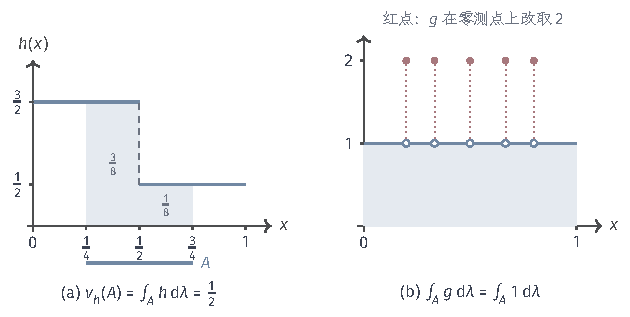
\includegraphics[width=106.684mm]{figures/02-abstract-mathematics/01-metric-and-measure/tikz/c4-weighted-measure/figure.pdf}
  \caption{由密度构造测度，以及几乎处处版本。(a)参考测度为$[0,1]$上的长度，密度$h$在$[0,1/2)$上取$3/2$、在$[1/2,1]$上取$1/2$；集合$A=[1/4,3/4]$的质量$\nu_h(A)$是$A$上方的阴影面积$3/8+1/8=1/2$。(b)常数密度$1$与在若干零测点（示意有理点）上改取$2$的函数$g$给出同一测度，因为改动的位置不承载长度。}
  \label{fig:density-weighted-measure}
\end{figure}

因此，说“$h$是$\nu$相对于$\mu$的密度”时，应当把与$h$几乎处处相等的所有函数看作同一个对象的不同版本；关于密度的逐点断言，如“$h>0$”“$h<\infty$”，都只在$\mu$-几乎处处的意义下才有意义。

\paragraph{正向结论与唯一性}
上面证明的是正向结论：几乎处处相等的函数产生同一个测度。密度的唯一性是反向的命题：若$h$与$g$产生同一个测度，能否推出它们几乎处处相等？这需要额外的有限性条件。取单点空间$X=\{0\}$，$\mu(\{0\})=+\infty$，$\nu=\mu$。常数$1$与常数$2$都满足$\int_{\{0\}}h\,\mathrm d\mu=+\infty=\nu(\{0\})$，可它们在一个$\mu$测度为$+\infty$的集合上不同。这里$\mu$不是$\sigma$有限的。第~\ref{sec:density-existence}节将在$\sigma$有限的条件下证明唯一性；在那之前，我们不对任意无限测度宣称密度唯一。

\section{密度的存在性}
\label{sec:density-existence}

上一节得到一个必要条件：$\nu$若有相对于$\mu$的密度，就必有$\nu\ll\mu$。本节证明，在两个测度都$\sigma$有限时这个条件也是充分的，并且密度在$\mu$-几乎处处意义下唯一。然后把这个结论用到第~\ref{sec:measure-decomposition}节的Lebesgue分解上，看清一个测度中哪一部分能用密度表示、哪一部分不能；最后把密度推广到有限有符号测度。

\subsection{Radon–Nikodym定理}
\label{sec:density-radon-nikodym}

绝对连续只是一个关于零测集的条件：$\mu$看不见的集合，$\nu$也看不见。它并没有直接给出任何函数。要从$\nu$在所有集合上的质量中“反求”一个逐点权重，必须同时满足不可数多个集合上的等式，这正是定理的难处。

\begin{theorem}[Radon–Nikodym定理]
\label{thm:density-radon-nikodym}
设$\mu,\nu$是可测空间$(X,\mathcal A)$上的$\sigma$有限非负测度，且$\nu\ll\mu$。则存在可测函数$h:X\to[0,+\infty)$，使
\[
 \nu(A)=\int_Ah\,\mathrm d\mu,\qquad A\in\mathcal A .
\]
若可测函数$g:X\to[0,+\infty]$也满足这一等式，则$g=h$ $\mu$-几乎处处。
\end{theorem}

把\term{Radon–Nikodym定理}（Radon-Nikodym theorem）与定理~\ref{thm:density-weighted-measure}对照：那里从$h$出发得到测度，这里从测度出发得到$h$。结合两者，在$\sigma$有限范围内，“$\nu$相对于$\mu$有密度”与“$\nu\ll\mu$”是同一件事。证明先处理两个测度都有限的情形，再用$\sigma$有限性把空间切成可数个有限块。

\paragraph{有限情形：候选权重取最大}
思路是在所有“不超过$\nu$”的权重中找一个最大的。直观上，若某个权重在每个集合上产生的质量都不超过$\nu$，而它已经大到不能再加高，那么它产生的质量就应该恰好等于$\nu$。

\begin{lemma}[有限测度的密度存在]
\label{lem:density-rn-finite}
设$\mu,\nu$是$(X,\mathcal A)$上的有限非负测度，且$\nu\ll\mu$。则存在可测函数$h:X\to[0,+\infty)$，使$\nu(A)=\int_Ah\,\mathrm d\mu$对一切$A\in\mathcal A$成立。
\end{lemma}

\begin{proof}
\emph{第一步：候选集合对取最大值封闭。}令
\[
 \mathcal G=\Bigl\{g:X\to[0,+\infty]\text{ 可测}:\ \int_Ag\,\mathrm d\mu\le\nu(A)\ \text{对一切}A\in\mathcal A\Bigr\}.
\]
$0\in\mathcal G$，所以$\mathcal G$非空。设$g_1,g_2\in\mathcal G$，$g=\max(g_1,g_2)$。对任意$A$，令$A_1=A\cap\{g_1\ge g_2\}$，$A_2=A\cap\{g_1<g_2\}$，二者可测、不交且并为$A$。在$A_1$上$g=g_1$，在$A_2$上$g=g_2$，于是
\[
 \int_Ag\,\mathrm d\mu=\int_{A_1}g_1\,\mathrm d\mu+\int_{A_2}g_2\,\mathrm d\mu\le\nu(A_1)+\nu(A_2)=\nu(A),
\]
故$g\in\mathcal G$。归纳可知有限个候选的最大值仍是候选。

\emph{第二步：用单调序列达到上确界。}令$s=\sup_{g\in\mathcal G}\int_Xg\,\mathrm d\mu$。每个候选满足$\int_Xg\,\mathrm d\mu\le\nu(X)$，所以$s\le\nu(X)<\infty$。取$g_n\in\mathcal G$使$\int_Xg_n\,\mathrm d\mu\to s$，再令$h_n=\max(g_1,\dots,g_n)$。由第一步$h_n\in\mathcal G$；$h_n$关于$n$单调递增，且$h_n\ge g_n$，所以$\int_Xg_n\,\mathrm d\mu\le\int_Xh_n\,\mathrm d\mu\le s$。令$h=\lim_nh_n$，它是可测函数。对每个$A$，$h_n\mathbf 1_A$递增到$h\mathbf 1_A$，单调收敛定理给出
\[
 \int_Ah\,\mathrm d\mu=\lim_{n\to\infty}\int_Ah_n\,\mathrm d\mu\le\nu(A),
\]
所以$h\in\mathcal G$；取$A=X$并由夹逼得$\int_Xh\,\mathrm d\mu=s$。上确界由一个候选达到，只用到了可数个候选，这正是单调收敛定理能够处理的情形。由于$\int_Xh\,\mathrm d\mu<\infty$，$h$只在一个$\mu$零测集上取$+\infty$；把这些值改为$0$不改变任何集合上的积分（第~\ref{sec:density-ae-version}小节），所以可设$h$处处有限。

\emph{第三步：剩余质量为零。}令$r(A)=\nu(A)-\int_Ah\,\mathrm d\mu$。因$h\in\mathcal G$，$r(A)\ge0$；$\nu$与$\nu_h$（定理~\ref{thm:density-weighted-measure}）都是有限测度，两个收敛级数逐项相减，可知$r$可数可加，是有限非负测度；又$r(A)\le\nu(A)$，所以$r\ll\mu$。反设$r(X)>0$。由$r\ll\mu$知$\mu(X)>0$，取
\[
 \varepsilon=\frac{r(X)}{2\mu(X)}>0,
\]
则$(r-\varepsilon\mu)(X)=r(X)/2>0$。$r-\varepsilon\mu$是两个有限测度之差，是有限有符号测度（定义~\ref{def:measure-signed}）。由Hahn分解（定理~\ref{thm:measure-hahn}），存在可测集$P$，使$P$是$r-\varepsilon\mu$的正集，$N=X\setminus P$是负集。

先说明$P$不是$\mu$零测集。$(r-\varepsilon\mu)(N)\le0$，所以$(r-\varepsilon\mu)(P)\ge(r-\varepsilon\mu)(X)>0$，从而$r(P)>\varepsilon\mu(P)\ge0$；再由$r\ll\mu$得$\mu(P)>0$。再说明在$h$上加高$\varepsilon\mathbf 1_P$仍是候选。对任意$A$，$A\cap P$是正集$P$的可测子集，于是$\varepsilon\mu(A\cap P)\le r(A\cap P)\le r(A)$，进而
\[
 \int_A(h+\varepsilon\mathbf 1_P)\,\mathrm d\mu=\int_Ah\,\mathrm d\mu+\varepsilon\mu(A\cap P)\le\int_Ah\,\mathrm d\mu+r(A)=\nu(A).
\]
所以$h+\varepsilon\mathbf 1_P\in\mathcal G$，但它的总积分为$s+\varepsilon\mu(P)>s$，与$s$是上确界矛盾。因此$r(X)=0$；由$0\le r(A)\le r(X)$，$r$在每个集合上为零，即$\nu(A)=\int_Ah\,\mathrm d\mu$。
\end{proof}

图~\ref{fig:density-rn-candidate}用一个事后已知密度$f$的例子示意第三步。蓝色候选$h$在左半段低于$f$，两者之间的黄色区域是尚未被表示的剩余质量$r$。Hahn分解找出的正集$P$，正是剩余质量“至少有$\varepsilon$倍长度”的地方；在那里把$h$加高$\varepsilon$，绿色条带仍在$f$之下，所以加高后仍是候选。只要剩余质量不为零，就总能这样再加高一点，最大的候选因而不留下任何剩余。

\begin{figure}[!htbp]
  \centering
  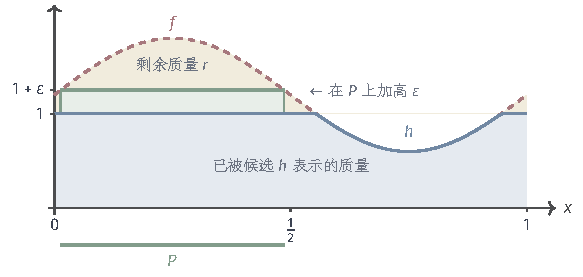
\includegraphics[width=98.771mm]{figures/02-abstract-mathematics/01-metric-and-measure/tikz/c4-rn-candidate/figure.pdf}
  \caption{有限情形证明第三步的示意。参考测度为$[0,1]$上的长度，目标测度的密度$f(x)=1.2+0.6\sin(2\pi x)$（红色虚线）在证明中事先未知，这里画出只为便于观察。候选$h=\min(f,1)$（蓝色实线）之下的质量已被表示，$h$与$f$之间的黄色区域是剩余质量$r$。取$\varepsilon=0.25$，正集$P=\{f-h\ge\varepsilon\}$约为$[0.013,0.487]$；在$P$上加高$\varepsilon$的绿色条带仍在$f$之下，所以$h+\varepsilon\mathbf 1_P$仍是候选而总积分更大。}
  \label{fig:density-rn-candidate}
\end{figure}

\paragraph{$\sigma$有限情形与唯一性}
有限情形中，$\nu(X)<\infty$保证了上确界$s$有限，$\mu(X)<\infty$保证了$r-\varepsilon\mu$是有限有符号测度，从而可以用Hahn分解。对$\sigma$有限测度，先把空间切成两种测度都有限的小块。

\begin{proof}[定理~\ref{thm:density-radon-nikodym}的证明]
\emph{有限分块。}由$\sigma$有限性，存在两两不交的可测集$A_1,A_2,\dots$覆盖$X$且$\mu(A_i)<\infty$，以及两两不交的可测集$B_1,B_2,\dots$覆盖$X$且$\nu(B_j)<\infty$。集合族$\{A_i\cap B_j\}_{i,j}$可数、两两不交、覆盖$X$，并且每块上$\mu$与$\nu$都有限；把它们排成一列$X_1,X_2,\dots$。

\emph{存在性。}对每个$k$，令$\mu_k(A)=\mu(A\cap X_k)$，$\nu_k(A)=\nu(A\cap X_k)$。它们是有限测度，且$\mu_k(A)=0$时$\nu(A\cap X_k)=0$，即$\nu_k\ll\mu_k$。由引理~\ref{lem:density-rn-finite}，存在有限值可测函数$h_k$使$\nu_k(A)=\int_Ah_k\,\mathrm d\mu_k$。对非负可测$f$有$\int_Xf\,\mathrm d\mu_k=\int_Xf\mathbf 1_{X_k}\,\mathrm d\mu$：对示性函数$f=\mathbf 1_B$，两边都是$\mu(B\cap X_k)$；由线性性推广到非负简单函数，再由简单函数逼近（引理~\ref{lem:integral-simple-approx}）和单调收敛推广到一般非负可测函数。令
\[
 h=\sum_{k=1}^\infty h_k\mathbf 1_{X_k},
\]
因各$X_k$不交，每点处至多一项非零，$h$有限、可测。对任意$A$，由$\nu$的可数可加性和非负级数的逐项积分（单调收敛定理），
\[
 \nu(A)=\sum_{k=1}^\infty\nu(A\cap X_k)=\sum_{k=1}^\infty\int_Ah_k\mathbf 1_{X_k}\,\mathrm d\mu=\int_A\sum_{k=1}^\infty h_k\mathbf 1_{X_k}\,\mathrm d\mu=\int_Ah\,\mathrm d\mu .
\]

\emph{唯一性。}设$g:X\to[0,+\infty]$也满足$\nu(A)=\int_Ag\,\mathrm d\mu$。固定$k$。由于$\int_{X_k}h\,\mathrm d\mu=\int_{X_k}g\,\mathrm d\mu=\nu(X_k)<\infty$，$h\mathbf 1_{X_k}$与$g\mathbf 1_{X_k}$都可积。令$D=X_k\cap\{h>g\}$，则$\int_Dh\,\mathrm d\mu=\nu(D)=\int_Dg\,\mathrm d\mu$，两边有限，由可积函数积分的线性性，
\[
 \int_X(h-g)\mathbf 1_D\,\mathrm d\mu=0 .
\]
在$D$上$g<h<\infty$，所以被积函数$(h-g)\mathbf 1_D$有定义且非负；积分为零的非负函数几乎处处为零（第~\ref{sec:integral-properties}节）；而它在$D$上严格为正，所以$\mu(D)=0$。同理$\mu(X_k\cap\{g>h\})=0$。对$k$取可数并，$\{g\ne h\}$是$\mu$零测集。
\end{proof}

整个证明只用到第~\ref{chap:measures}章的测度运算与Hahn分解，以及第~\ref{chap:integration}章的积分基本性质和单调收敛定理，不需要函数空间的理论。从第二步还能读出密度的一个刻画：$\mathrm d\nu/\mathrm d\mu$是所有“在每个集合上都不超过$\nu$”的权重中积分最大的那个。

\subsection{密度表示与测度分解}
\label{sec:density-decomposition}

第~\ref{sec:measure-decomposition}节已经把一个$\sigma$有限测度$\nu$相对于参考测度$\mu$唯一地拆成$\nu=\nu_{\mathrm{ac}}+\nu_{\mathrm s}$，其中$\nu_{\mathrm{ac}}\ll\mu$、$\nu_{\mathrm s}\perp\mu$（定理~\ref{thm:measure-lebesgue-decomposition}）。那里只分开了两种质量，没有给绝对连续部分任何函数表示；Radon–Nikodym定理正好补上这一步。

\begin{theorem}[Lebesgue分解的密度形式（推论）]
\label{thm:density-lebesgue-form}
设$\mu,\nu$是$(X,\mathcal A)$上的$\sigma$有限非负测度。则存在可测函数$h:X\to[0,+\infty)$和非负测度$\nu_{\mathrm s}\perp\mu$，使
\[
 \nu(A)=\int_Ah\,\mathrm d\mu+\nu_{\mathrm s}(A),\qquad A\in\mathcal A,
\]
其中$\nu_{\mathrm s}$唯一，$h$在$\mu$-几乎处处意义下唯一。特别地，$\nu$相对于$\mu$有密度，当且仅当$\nu_{\mathrm s}=0$。
\end{theorem}

\begin{proof}
由定理~\ref{thm:measure-lebesgue-decomposition}得到$\nu=\nu_{\mathrm{ac}}+\nu_{\mathrm s}$。$\nu_{\mathrm{ac}}(A)\le\nu(A)$，所以覆盖$X$且$\nu$有限的可数块也使$\nu_{\mathrm{ac}}$有限，$\nu_{\mathrm{ac}}$是$\sigma$有限的。对$\nu_{\mathrm{ac}}\ll\mu$应用定理~\ref{thm:density-radon-nikodym}，得$h=\mathrm d\nu_{\mathrm{ac}}/\mathrm d\mu$。唯一性：若另有$(h',\nu_{\mathrm s}')$满足同样的表示，则$A\mapsto\int_Ah'\,\mathrm d\mu$绝对连续（定理~\ref{thm:density-weighted-measure}），由Lebesgue分解的唯一性，它等于$\nu_{\mathrm{ac}}$且$\nu_{\mathrm s}'=\nu_{\mathrm s}$；再由Radon–Nikodym定理中的唯一性得$h'=h$ $\mu$-几乎处处。最后，若$\nu$有密度，则$\nu\ll\mu$，$\nu=\nu+0$就是它的Lebesgue分解，所以$\nu_{\mathrm s}=0$；反之$\nu_{\mathrm s}=0$时$h$就是$\nu$的密度。
\end{proof}

两个定理的分工由此清楚：Lebesgue分解只用测度把参考测度能看见的质量与看不见的质量分开；Radon–Nikodym定理为前一部分找到逐点权重。奇异部分无论如何也写不成相对于$\mu$的密度，因为它集中在一个$\mu$零测集上，而任何密度在零测集上的积分都是$0$。

\paragraph{实轴上的三种质量}
以Lebesgue测度$\lambda$为参考时，第~\ref{sec:measure-decomposition}节把奇异部分进一步拆成点质量与没有点质量的奇异连续质量。考虑$[0,1]$上的概率测度
\[
 \nu=\tfrac12\lambda|_{[0,1]}+\tfrac14\delta_{1/2}+\tfrac14\mu_C,
\]
其中$\mu_C$是第~\ref{sec:measure-decomposition}节的Cantor测度，集中在Lebesgue零测的Cantor集$C$上。$\tfrac14\delta_{1/2}+\tfrac14\mu_C$集中在零测集$C\cup\{1/2\}$上，与$\lambda$相互奇异；$\tfrac12\lambda|_{[0,1]}$相对于$\lambda$绝对连续。由分解的唯一性，
\[
 \nu(A)=\int_A\tfrac12\mathbf 1_{[0,1]}\,\mathrm d\lambda+\tfrac14\delta_{1/2}(A)+\tfrac14\mu_C(A).
\]
图~\ref{fig:density-lebesgue-form}画出这三部分：只有高为$1/2$的蓝色区域是密度能表示的，红色箭头和绿色Cantor集上的质量都在密度之外。

\begin{figure}[!htbp]
  \centering
  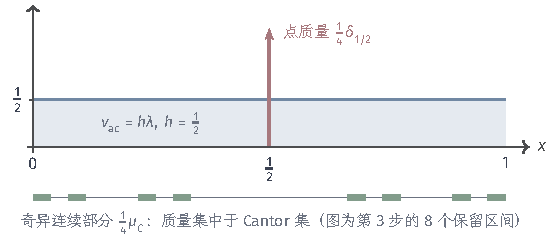
\includegraphics[width=94.365mm]{figures/02-abstract-mathematics/01-metric-and-measure/tikz/c4-lebesgue-density/figure.pdf}
  \caption{相对于长度测度的密度只表示绝对连续部分。$\nu=\tfrac12\lambda|_{[0,1]}+\tfrac14\delta_{1/2}+\tfrac14\mu_C$：蓝色区域是密度$h=1/2$表示的质量$1/2$；红色箭头是位于$1/2$的点质量$1/4$；下方绿色线段是Cantor集构造第$3$步保留的$8$个区间，Cantor测度的质量$1/4$集中在它们的极限——零长度的Cantor集上。后两部分都集中在长度零测集上，任何密度都无法表示。}
  \label{fig:density-lebesgue-form}
\end{figure}

由定理~\ref{thm:density-lebesgue-form}，$\nu$整体具有Lebesgue密度，当且仅当点质量部分与奇异连续部分都为零。累计函数$F(x)=\nu((-\infty,x])$的跳跃恰好读出点质量（第~\ref{sec:measure-construction}节），所以“$F$连续”只能排除点质量。Cantor测度的累计函数就是处处连续的Cantor函数，它却没有密度。判断密度是否存在，应当检查绝对连续性，而不是累计函数的连续性；第~\ref{sec:density-increment}小节还会从函数一侧回到这一点。

\paragraph{有限性条件不能随意去掉}
在$[0,1]$的Borel可测空间上取计数测度$c$与Lebesgue测度$\lambda$。$c(A)=0$只在$A=\varnothing$时成立，所以$\lambda\ll c$。若存在可测$h\ge0$使$\lambda(A)=\int_Ah\,\mathrm dc$，取$A=\{x\}$，$h\mathbf 1_{\{x\}}=h(x)\mathbf 1_{\{x\}}$是简单函数，于是
\[
 0=\lambda(\{x\})=h(x)\,c(\{x\})=h(x),\qquad x\in[0,1].
\]
$h$处处为零，却要给出$\lambda([0,1])=1$，矛盾。所以$\lambda$没有相对于$c$的密度。定理失效的原因在于参考测度：$c$的有限测度集只能是有限集，可数个有限集的并仍是可数集，盖不住$[0,1]$，所以$c$不是$\sigma$有限的。$\lambda$本身有限，第~\ref{sec:measure-decomposition}节的Lebesgue分解对它照常成立，给出$\lambda_{\mathrm{ac}}=\lambda$、$\lambda_{\mathrm s}=0$；失败的只是“为绝对连续部分找函数”这一步。

\begin{figure}[!htbp]
  \centering
  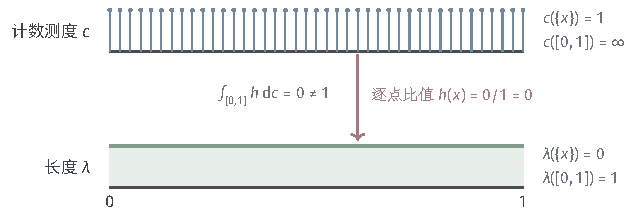
\includegraphics[width=107.636mm]{figures/02-abstract-mathematics/01-metric-and-measure/tikz/c4-counting-counterexample/figure.pdf}
  \caption{参考测度不$\sigma$有限时密度可能不存在。上方的计数测度$c$给$[0,1]$中每一点质量$1$（图中只画出若干点），下方的长度$\lambda$给单点质量$0$、给整个区间质量$1$。若$\lambda$有相对于$c$的密度，逐点比较单点质量迫使密度处处为$0$，其积分为$0$，不能恢复$\lambda([0,1])=1$。}
  \label{fig:density-counting-counterexample}
\end{figure}

这个反例说明定理不能无条件推广，但不说明$\sigma$有限是密度存在的必要条件。仍以不$\sigma$有限的$c$为参考，$\delta_0$有密度$\mathbf 1_{\{0\}}$：$\int_A\mathbf 1_{\{0\}}\,\mathrm dc=c(A\cap\{0\})=\delta_0(A)$。$\sigma$有限是本章采用的一组充分条件。图~\ref{fig:density-counting-counterexample}直观地显示了反例中失败的原因：参考测度的质量分得太“碎”，每一点都有正质量，任何逐点权重都只能逐点地复制目标测度在单点上的质量，而$\lambda$的质量恰恰不在任何单点上。

\subsection{有符号测度的密度}
\label{sec:density-signed}

第~\ref{sec:measure-signed}节的有限有符号测度允许集合质量为负。它同样可以用一个函数表示，只不过这个函数可以取负值，正负部分别对应Jordan分解的两项。

\begin{theorem}[有符号测度的密度]
\label{thm:density-signed}
设$\mu$是$(X,\mathcal A)$上的$\sigma$有限非负测度，$\eta$是有限有符号测度。则$|\eta|\ll\mu$当且仅当存在$\mu$可积的实值函数$h$，使
\[
 \eta(A)=\int_Ah\,\mathrm d\mu,\qquad A\in\mathcal A .
\]
此时$h$在$\mu$-几乎处处意义下唯一，并且对一切$A\in\mathcal A$，
\[
 \eta^+(A)=\int_Ah^+\,\mathrm d\mu,\qquad \eta^-(A)=\int_Ah^-\,\mathrm d\mu,\qquad |\eta|(A)=\int_A|h|\,\mathrm d\mu,
\]
其中$h^+=\max(h,0)$，$h^-=\max(-h,0)$。
\end{theorem}

\begin{proof}
设$|\eta|\ll\mu$。由Jordan分解（定理~\ref{thm:measure-jordan}），$\eta=\eta^+-\eta^-$，且$\eta^\pm\le\eta^++\eta^-=|\eta|$（定义~\ref{def:measure-total-variation}），所以$\eta^\pm\ll\mu$。$\eta^\pm$是有限测度，当然$\sigma$有限；由定理~\ref{thm:density-radon-nikodym}，存在有限值密度$h_1=\mathrm d\eta^+/\mathrm d\mu$与$h_2=\mathrm d\eta^-/\mathrm d\mu$，且$\int_Xh_1\,\mathrm d\mu=\eta^+(X)<\infty$，$h_2$同理，二者都可积。令$h=h_1-h_2$，由可积函数积分的线性性，$\eta(A)=\int_Ah_1\,\mathrm d\mu-\int_Ah_2\,\mathrm d\mu=\int_Ah\,\mathrm d\mu$。

反过来，设$\eta(A)=\int_Ah\,\mathrm d\mu$且$h$可积。令$P=\{h\ge0\}$，$N=\{h<0\}$。对$P$的任意可测子集$A$，$\eta(A)=\int_Ah\,\mathrm d\mu\ge0$；对$N$的任意可测子集，$\eta(A)\le0$。所以$(P,N)$是$\eta$的一组Hahn分解，由Jordan分解得
\[
 \begin{aligned}
  \eta^+(A)&=\eta(A\cap P)=\int_Ah\mathbf 1_{\{h\ge0\}}\,\mathrm d\mu=\int_Ah^+\,\mathrm d\mu,\\
  \eta^-(A)&=-\eta(A\cap N)=\int_Ah^-\,\mathrm d\mu,
 \end{aligned}
\]
相加得$|\eta|(A)=\int_A(h^++h^-)\,\mathrm d\mu=\int_A|h|\,\mathrm d\mu$。由定理~\ref{thm:density-weighted-measure}，$|\eta|\ll\mu$。这一段对前一段构造的$h$同样适用，所以三个公式在必要性方向也成立。

唯一性：若可积的$h,g$都表示$\eta$，则对$D=\{h>g\}$有$\int_X(h-g)\mathbf 1_D\,\mathrm d\mu=\eta(D)-\eta(D)=0$，非负被积函数几乎处处为零，所以$\mu(D)=0$；同理$\mu(\{g>h\})=0$。
\end{proof}

定理把集合层面的正负分解翻译成函数层面的正负部分：Hahn分解的正区域可以取为$\{h\ge0\}$，Jordan的两项就是$h$的正部与负部分别产生的测度，这与第~\ref{chap:integration}章用正负部定义实值函数积分的做法一致。总变差对应$|h|$的积分，所以“$\eta$有有限总变差且对$\mu$绝对连续”恰好对应“密度绝对可积”。

\paragraph{抵消与总变差}
在$[0,1]$上取$\mu=\lambda|_{[0,1]}$与$h(x)=1-2x$，令$\eta(A)=\int_Ah\,\mathrm d\lambda$。整体上$\eta([0,1])=\int_0^1(1-2x)\,\mathrm dx=0$，正负质量完全抵消。由定理，正区域为$[0,1/2]$，
\[
 \eta^+([0,1])=\int_0^{1/2}(1-2x)\,\mathrm dx=\tfrac14,\qquad \eta^-([0,1])=\int_{1/2}^1(2x-1)\,\mathrm dx=\tfrac14,
\]
所以$|\eta|([0,1])=\int_0^1|1-2x|\,\mathrm dx=\tfrac12$。$\eta(X)=0$并不说明$\eta$处处为零，总变差记录了被抵消掉的变化总量。第~\ref{sec:density-increment}小节将用这个定理表示由函数增量产生的有符号测度。

\section{密度的运算规则}
\label{sec:density-rules}

有了密度以后，最常用的操作是“换参考测度”：同一个函数对目标测度的积分，改写成对参考测度的加权积分；几个测度相对于同一参考的密度相加；或者经过一个中间测度连续换两次参考。本节依次建立这些规则，并对每条规则注明所需的测度关系，以及等式在哪个测度的几乎处处意义下成立。

\subsection{换测度公式}
\label{sec:density-change-of-measure}

密度的定义\eqref{eq:density-definition}只说明示性函数$\mathbf 1_A$对$\nu$的积分等于$\mathbf 1_Ah$对$\mu$的积分。积分的构造本来就是从示性函数出发，经简单函数和单调逼近推广到一般函数的，所以这个等式可以沿同一条路线推广。

\begin{theorem}[换测度公式]
\label{thm:density-change-of-measure}
设$\mu,\nu$是$(X,\mathcal A)$上的非负测度，$h$是$\nu$相对于$\mu$的密度。约定$0\cdot(+\infty)=0$。
\begin{enumerate}
 \item 对每个可测函数$f:X\to[0,+\infty]$，
 \[
  \int_Xf\,\mathrm d\nu=\int_Xfh\,\mathrm d\mu .
 \]
 \item 对实值或复值可测函数$f$，$f$对$\nu$可积当且仅当$fh$对$\mu$可积，此时上式仍成立。
\end{enumerate}
\end{theorem}

\begin{proof}
(1) 对$f=\mathbf 1_A$，左边是$\nu(A)$，右边是$\int_Ah\,\mathrm d\mu$，二者由密度的定义相等。对非负简单函数$f=\sum_ic_i\mathbf 1_{A_i}$，两边对$f$都是线性的（非负积分的线性性），所以等式成立。对一般非负可测$f$，取非负简单函数列$s_n\uparrow f$（引理~\ref{lem:integral-simple-approx}）。因$h\ge0$，$s_nh$也单调递增并逐点收敛到$fh$。对两边分别用单调收敛定理，
\[
 \int_Xf\,\mathrm d\nu=\lim_{n\to\infty}\int_Xs_n\,\mathrm d\nu=\lim_{n\to\infty}\int_Xs_nh\,\mathrm d\mu=\int_Xfh\,\mathrm d\mu .
\]
两边允许同时为$+\infty$。

(2) 对$|f|$用(1)，得$\int_X|f|\,\mathrm d\nu=\int_X|f|h\,\mathrm d\mu=\int_X|fh|\,\mathrm d\mu$，所以两种可积性等价。设$f$实值且可积，则$(fh)^\pm=f^\pm h$，对$f^+$与$f^-$分别用(1)，两边各得两个有限数，相减即得等式。复值时对实部和虚部分别使用实值情形。
\end{proof}

\term{换测度公式}（change-of-measure formula）把“对目标测度累计”改写成“对参考测度加权累计”。例如$[0,1]$上$\nu$相对于长度的密度为$h(x)=2x$，取$f(x)=x$，则
\[
 \int_{[0,1]}f\,\mathrm d\nu=\int_0^1x\cdot2x\,\mathrm dx=\frac23 .
\]
若$\nu$是概率测度，这就是用概率密度计算期望的公式。证明中没有用到任何有限性条件：只要密度存在，换测度公式就成立。

\paragraph{与推前换元的区别}
第~\ref{sec:integral-change-of-variables}节的推前公式（定理~\ref{thm:integral-pushforward-change}）
\[
 \int_Yg\,\mathrm d(T_\#\mu)=\int_Xg\circ T\,\mathrm d\mu
\]
也是一种“换测度”，但它改变的是所在空间：点经映射$T$从$X$搬到$Y$，被积函数相应地复合上$T$。换测度公式则留在同一空间$X$上，点不移动，被积函数不变，只是每一处的权重乘上$h$。两种操作可以接连使用：若推前测度$T_\#\mu$有相对于参考测度的密度$q$，那么先推前再换测度，就把$X$上的积分化为$Y$上的加权积分$\int_Ygq\,\mathrm d\lambda$。第~\ref{sec:density-pushforward}小节正是这样计算推前测度的密度。

\subsection{密度的线性组合}
\label{sec:density-linear}

\paragraph{共同参考测度下的加法}
设$\nu_1,\dots,\nu_m$相对于同一个参考测度$\mu$分别有密度$h_1,\dots,h_m$，$a_1,\dots,a_m\ge0$。由非负积分的线性性，对每个可测集$A$，
\[
 \sum_{i=1}^ma_i\nu_i(A)=\sum_{i=1}^ma_i\int_Ah_i\,\mathrm d\mu=\int_A\sum_{i=1}^ma_ih_i\,\mathrm d\mu,
\]
所以$\sum_ia_i\nu_i$的密度是$\sum_ia_ih_i$。这里关键是参考测度相同：密度是相对于参考的换算比例，只有同一种参考下的比例才能直接相加，正如以不同货币计价的价格不能直接相加。

\paragraph{差与有限性}
对差的处理要谨慎。若$\nu_1,\nu_2$是有限测度，则$h_1,h_2$可积，$\eta=a\nu_1-b\nu_2$（$a,b$为实数）是有限有符号测度，由可积函数积分的线性性，它的密度是可积函数$ah_1-bh_2$，与定理~\ref{thm:density-signed}一致。对无限测度不能这样做：在$\mathbb R$上取$\nu_1=\nu_2=\lambda$，形式上$h_1-h_2=0$，可$\nu_1(\mathbb R)-\nu_2(\mathbb R)=\infty-\infty$没有定义，所以“$\nu_1-\nu_2$”根本不是一个在所有集合上都有值的对象，不能仅凭密度相减就宣称它的密度为$0$。

\paragraph{混合测度的统一表示}
共同参考测度也能用来表示一个相对于长度没有密度的测度。在$[0,1]$上取参考测度$\mu=\lambda|_{[0,1]}+\delta_0$。先计算两个分量相对于$\mu$的密度。对可测集$A\subseteq[0,1]$，
\[
 \begin{aligned}
  \int_A\mathbf 1_{(0,1]}\,\mathrm d\mu&=\lambda(A\cap(0,1])+\delta_0(A\cap(0,1])=\lambda(A),\\
  \int_A\mathbf 1_{\{0\}}\,\mathrm d\mu&=\lambda(A\cap\{0\})+\delta_0(A\cap\{0\})=\delta_0(A),
 \end{aligned}
\]
其中第一式用了$\lambda(\{0\})=0$与$0\notin(0,1]$，第二式用了$\lambda(\{0\})=0$。所以$\mathrm d\lambda|_{[0,1]}/\mathrm d\mu=\mathbf 1_{(0,1]}$，$\mathrm d\delta_0/\mathrm d\mu=\mathbf 1_{\{0\}}$。由线性组合规则，$a,b\ge0$时
\[
 \nu=a\lambda|_{[0,1]}+b\delta_0,\qquad \frac{\mathrm d\nu}{\mathrm d\mu}=a\mathbf 1_{(0,1]}+b\mathbf 1_{\{0\}},
\]
总质量$\nu([0,1])=a+b$。当$b>0$时$\nu$在长度零测集$\{0\}$上有正质量，整体没有Lebesgue密度；换用共同参考$\mu$后，点质量与长度质量就能由一个函数统一表示。图~\ref{fig:density-mixed-reference}取$a=3/4$、$b=1/4$。

\begin{figure}[!htbp]
  \centering
  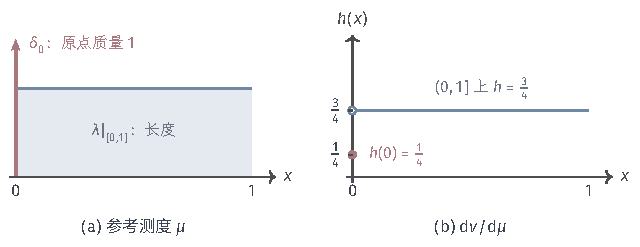
\includegraphics[width=108.433mm]{figures/02-abstract-mathematics/01-metric-and-measure/tikz/c4-mixed-reference/figure.pdf}
  \caption{在共同参考测度下统一表示混合测度。(a)参考测度$\mu=\lambda|_{[0,1]}+\delta_0$由区间上的长度（蓝色）和原点的单位点质量（红色箭头）组成。(b)$\nu=\tfrac34\lambda|_{[0,1]}+\tfrac14\delta_0$相对于$\mu$的密度：在$(0,1]$上取$3/4$，在原点取$1/4$（红色实心点）；原点处的值有意义，因为原点在$\mu$下有正质量。}
  \label{fig:density-mixed-reference}
\end{figure}

图中原点处的密度值$1/4$不能随意改动：原点在$\mu$下质量为$1$，不是$\mu$零测集。这与第~\ref{sec:density-ae-version}小节的长度参考不同，那里单点上的取值可以任意改变。哪些点上的取值有意义，取决于参考测度在那里有没有质量。

\subsection{密度的链式规则}
\label{sec:density-chain-rule}

换算比例可以连乘：先从一种参考换到中间测度，再从中间测度换到目标。为避免与Lebesgue测度的记号冲突，本小节用$\rho$表示最底层的参考测度。

\begin{theorem}[密度的链式规则]
\label{thm:density-chain-rule}
设$\rho,\mu,\nu$是$(X,\mathcal A)$上的$\sigma$有限非负测度，且$\nu\ll\mu\ll\rho$。则$\nu\ll\rho$，并且
\[
 \frac{\mathrm d\nu}{\mathrm d\rho}=\frac{\mathrm d\nu}{\mathrm d\mu}\cdot\frac{\mathrm d\mu}{\mathrm d\rho}\qquad\rho\text{-几乎处处}.
\]
\end{theorem}

\begin{proof}
由Radon–Nikodym定理，取$g=\mathrm d\nu/\mathrm d\mu$与$k=\mathrm d\mu/\mathrm d\rho$。对任意可测集$A$，先用$g$的定义，再对非负函数$\mathbf 1_Ag$与密度$k$使用换测度公式，
\[
 \nu(A)=\int_X\mathbf 1_Ag\,\mathrm d\mu=\int_X\mathbf 1_Agk\,\mathrm d\rho=\int_Agk\,\mathrm d\rho .
\]
所以$gk$是$\nu$相对于$\rho$的一个密度，由定理~\ref{thm:density-weighted-measure}得$\nu\ll\rho$。$\nu,\rho$都$\sigma$有限，由Radon–Nikodym定理中的唯一性，任何版本的$\mathrm d\nu/\mathrm d\rho$都与$gk$ $\rho$-几乎处处相等。
\end{proof}

这条规则称为\term{密度的链式规则}（chain rule for densities），它与一元微积分的链式法则形式相似，但依据是集合质量的连续换算，而不是对坐标求导。图~\ref{fig:density-chain-rule}给出一个数值例子。在$[0,1]$上取$\rho=\lambda|_{[0,1]}$，$\mathrm d\mu/\mathrm d\rho=2x$，$\mathrm d\nu/\mathrm d\mu=\tfrac32x$。链式规则给出$\mathrm d\nu/\mathrm d\lambda=3x^2$。可以直接核对：$\mu([0,1])=\int_0^12x\,\mathrm dx=1$，$\nu([0,1])=\int_0^1\tfrac32x\cdot2x\,\mathrm dx=\int_0^13x^2\,\mathrm dx=1$，两种算法在每个区间上都给出相同的值。

\begin{figure}[!htbp]
  \centering
  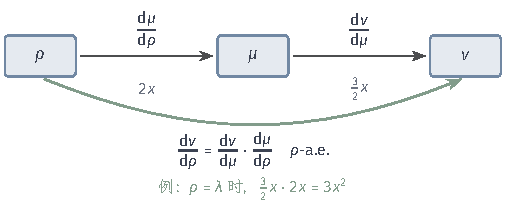
\includegraphics[width=85.651mm]{figures/02-abstract-mathematics/01-metric-and-measure/tikz/c4-chain-rule/figure.pdf}
  \caption{密度的链式规则。箭头表示“箭头终点的测度相对于起点测度的密度”：先从$\rho$换到$\mu$，再从$\mu$换到$\nu$，两段密度相乘就是从$\rho$直接换到$\nu$的密度（绿色弧线），等式在$\rho$-几乎处处意义下成立。箭头下方是$[0,1]$上$\rho=\lambda$时的例子，$2x$与$\tfrac32x$相乘得到$3x^2$。}
  \label{fig:density-chain-rule}
\end{figure}

\paragraph{版本的选择}
$g=\mathrm d\nu/\mathrm d\mu$只确定到$\mu$零测集，而结论是关于$\rho$零测集的。两者并不冲突。设$g'$是$g$的另一个版本，$g\ne g'$只发生在某个$\mu$零测集$M$上。乘积$gk$与$g'k$只可能在$M\cap\{k>0\}$上不同。由$0=\mu(M)=\int_Mk\,\mathrm d\rho$，$k$在$M$上$\rho$-几乎处处为零，所以$\rho(M\cap\{k>0\})=0$。也就是说，在$k=0$处乘积按约定取$0$，与$g$的取值无关；在$k>0$处，$\mu$的零测例外也是$\rho$的零测例外。所以无论选哪个版本，乘积都给出同一个$\rho$-几乎处处确定的密度。

\subsection{等价测度与密度的倒数}
\label{sec:density-inverse}

若两个测度相互绝对连续，即等价（第~\ref{sec:measure-relations}节），就可以从任一方换到另一方。反向的密度应当是原密度的倒数，但这需要先保证原密度几乎处处既不为零也不为无穷。

\begin{theorem}[密度的倒数（推论）]
\label{thm:density-inverse}
设$\mu,\nu$是$(X,\mathcal A)$上的$\sigma$有限非负测度，$\nu\ll\mu$且$\mu\ll\nu$，$h=\mathrm d\nu/\mathrm d\mu$。则$0<h<\infty$ $\mu$-几乎处处，并且
\[
 \frac{\mathrm d\mu}{\mathrm d\nu}=\frac1h,
\]
等式在$\mu$-几乎处处意义下成立，也在$\nu$-几乎处处意义下成立。
\end{theorem}

\begin{proof}
由Radon–Nikodym定理可取有限值的$h$。令$Z=\{h=0\}$，则$\nu(Z)=\int_Zh\,\mathrm d\mu=0$；由$\mu\ll\nu$得$\mu(Z)=0$。所以$0<h<\infty$ $\mu$-几乎处处。定义$u=1/h$于$X\setminus Z$，$u=0$于$Z$。对任意可测集$A$，由换测度公式，
\[
 \int_Au\,\mathrm d\nu=\int_X\mathbf 1_Auh\,\mathrm d\mu=\mu(A\setminus Z)=\mu(A),
\]
所以$u$是$\mu$相对于$\nu$的密度。两个测度等价，零测集相同，因此$\mu$-几乎处处与$\nu$-几乎处处是同一回事。
\end{proof}

这个结论也可以从链式规则读出：对$\mu\ll\nu\ll\mu$用定理~\ref{thm:density-chain-rule}，得$(\mathrm d\mu/\mathrm d\nu)\cdot h=\mathrm d\mu/\mathrm d\mu=1$ $\mu$-几乎处处。例如$[0,1]$上$\nu$相对于$\lambda$的密度为$2x$，它只在零测集$\{0\}$上为零，所以$\nu$与$\lambda|_{[0,1]}$等价，反向密度为$1/(2x)$，$x\in(0,1]$。反向密度无界，但仍满足$\int_0^1\frac1{2x}\cdot2x\,\mathrm dx=1=\lambda([0,1])$。

\paragraph{单向绝对连续时的信息丢失}
若只有$\nu\ll\mu$，密度$h$可以在一个正$\mu$测度的区域上为零。取$\mu=\lambda|_{[0,2]}$，$\nu=\lambda|_{[0,1]}$，则$h=\mathbf 1_{[0,1]}$。在$(1,2]$上，$\mu$有质量$1$，$\nu$却为零，$1/h$在这里没有定义。更根本的是，$\nu$在$(1,2]$上看不到任何质量，所以无论用什么函数加权，$\int_{(1,2]}u\,\mathrm d\nu$都是$0$，不可能恢复$\mu((1,2])=1$：$\mu$并不相对于$\nu$绝对连续，反向密度不存在。图~\ref{fig:density-one-sided-loss}显示了这块被目标测度完全忽略的区域。倒数公式只能在两个测度等价的范围内使用。

\begin{figure}[!htbp]
  \centering
  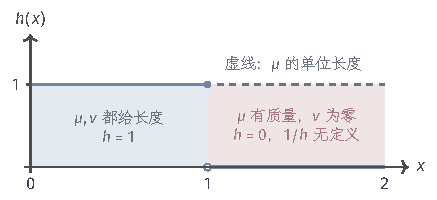
\includegraphics[width=73.914mm]{figures/02-abstract-mathematics/01-metric-and-measure/tikz/c4-one-sided-loss/figure.pdf}
  \caption{单向绝对连续时密度不能取倒数。参考测度$\mu$是$[0,2]$上的长度，目标测度$\nu$是$[0,1]$上的长度，密度$h=\mathbf 1_{[0,1]}$（蓝色实线）。在$[0,1]$上$h=1$，两种测度一致；在红色区域$(1,2]$上$h=0$，$\mu$有质量$1$而$\nu$没有质量，从$\nu$出发无法恢复这部分质量。}
  \label{fig:density-one-sided-loss}
\end{figure}

\section{密度的计算与表示}
\label{sec:density-computation}

前两节回答了密度何时存在、怎样使用。本节回到具体测度，依次计算三类常见对象的密度：可数集合上的离散质量、由实轴函数增量产生的质量，以及经过映射后得到的推前测度。每个例子都先指明参考测度，再求密度，最后核对它能否恢复目标测度在集合上的质量。

\subsection{离散测度的密度}
\label{sec:density-discrete}

\paragraph{逐点相除}
设$X=\{x_1,x_2,\dots\}$是可数集合，取全部子集为可测集，参考测度与目标测度分别为
\[
 \mu=\sum_im_i\delta_{x_i},\qquad \nu=\sum_ip_i\delta_{x_i},\qquad m_i,p_i\in[0,+\infty).
\]
单点质量有限，可数个单点覆盖$X$，所以两者都$\sigma$有限。先检查绝对连续：$\mu(A)=0$当且仅当$A$中每点的$m_i$都为零，所以$\nu\ll\mu$当且仅当“$m_i=0$蕴含$p_i=0$”。在此条件下，令
\[
 h(x_i)=\frac{p_i}{m_i}\quad(m_i>0),\qquad h(x_i)\text{ 取任意非负值}\quad(m_i=0).
\]
对离散测度的积分是加权求和（第~\ref{sec:integral-classical}节），于是对任意$A\subseteq X$，
\[
 \int_Ah\,\mathrm d\mu=\sum_{x_i\in A}h(x_i)m_i=\sum_{x_i\in A,\,m_i>0}p_i=\sum_{x_i\in A}p_i=\nu(A),
\]
第三个等号用到$m_i=0$时$p_i=0$。因此$h$是$\nu$相对于$\mu$的密度。$m_i=0$的点是$\mu$零测集，密度在那里的取值可以任意，这正是第~\ref{sec:density-ae-version}小节的几乎处处版本。与长度测度不同，离散参考测度在每个正质量点上都允许逐点相除，第~\ref{sec:density-definition}小节有限点集上的质量之比在这里推广到了可数情形。

\paragraph{同一分布换两种参考}
在$\{0,1,2,\dots\}$上取参数为$1$的Poisson分布$p_k=\mathrm e^{-1}/k!$为目标。相对于计数测度，密度就是概率质量函数$p_k$本身。若改用几何权重$m_k=2^{-(k+1)}$作参考，所有$m_k>0$，密度为
\[
 h(k)=\frac{p_k}{m_k}=\frac{2^{k+1}\mathrm e^{-1}}{k!},
\]
前几项约为$0.736,1.472,1.472,0.981,0.491,0.196$。核对一个集合：$\nu(\{0,1\})=2\mathrm e^{-1}\approx0.7358$，而$h(0)m_0+h(1)m_1\approx0.7358\cdot0.5+1.4715\cdot0.25\approx0.7358$。两种密度之间由链式规则联系：几何权重相对于计数测度的密度是$m_k$，所以$h(k)\cdot m_k=p_k$。图~\ref{fig:density-discrete}画出了两组点质量及它们的比值。

\begin{figure}[!htbp]
  \centering
  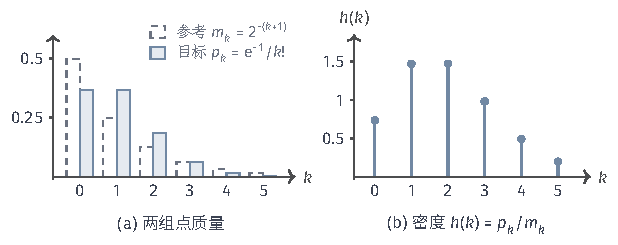
\includegraphics[width=104.712mm]{figures/02-abstract-mathematics/01-metric-and-measure/tikz/c4-discrete-density/figure.pdf}
  \caption{可数集合上的离散密度。(a)虚线框为几何参考质量$m_k=2^{-(k+1)}$，蓝色柱为Poisson目标质量$p_k=\mathrm e^{-1}/k!$，$k=0,\dots,5$。(b)密度$h(k)=p_k/m_k$：$k=1,2$处目标质量相对参考最多，$h$约为$1.47$；$k$增大后几何权重比阶乘倒数衰减得慢，$h$趋于零。}
  \label{fig:density-discrete}
\end{figure}

\paragraph{总质量}
密度的计算与总质量是否有限无关。仍以几何权重为参考，计数测度$\nu=\sum_k\delta_k$的密度是$h(k)=2^{k+1}$，$\nu$的总质量为$+\infty$，但每个有限集合上的质量都由$h$正确恢复。只有目标测度是概率测度时，才要求$\sum_kh(k)m_k=1$。

\subsection{增量测度的密度}
\label{sec:density-increment}

第~\ref{sec:integral-differentiation}节从函数一侧研究了增量：有界变差函数可以写成两个单调函数之差，绝对连续函数的增量可以由导数的积分恢复。本小节把函数增量变成集合上的质量，再问这个质量何时有Lebesgue密度。

\paragraph{由增量产生的有符号测度}
设$F:[a,b]\to\mathbb R$可以写成$F=F_1-F_2$，其中$F_1,F_2$单调不减且右连续。每个右连续的有界变差函数都有这样的分解：取$F_1(x)$为$F$在$[a,x]$上的总变差、$F_2=F_1-F$，二者单调不减（第~
ef{sec:integral-differentiation}节）；$F$右连续时$F_1$也右连续，这一点需要单独证明（可参照Folland《Real Analysis》第3.5节关于有界变差函数的讨论），本小节直接使用这一结论。把$F_j$延拓到$\mathbb R$，在$x<a$处取$F_j(a)$，在$x>b$处取$F_j(b)$，延拓后仍单调不减、右连续。由第~\ref{sec:measure-construction}节的Lebesgue–Stieltjes构造得到有限测度$\mu_{F_1},\mu_{F_2}$，它们都集中在$(a,b]$上。令
\[
 \eta_F(E)=\mu_{F_1}(E)-\mu_{F_2}(E),\qquad E\in\mathcal B((a,b]),
\]
则$\eta_F$是$(a,b]$上的有限有符号测度，并且对$a\le s<t\le b$有
\[
 \eta_F((s,t])=\bigl(F_1(t)-F_1(s)\bigr)-\bigl(F_2(t)-F_2(s)\bigr)=F(t)-F(s).
\]
称$\eta_F$为$F$的\term{增量测度}（increment measure）。区间取左开右闭，与右连续性配合：$\eta_F$给$(s,t]$的质量是右端点值减左端点值。$F(a)$本身不进入$\eta_F$，它是恢复$F$时需要单独记下的常数：$F(x)=F(a)+\eta_F((a,x])$。

$\eta_F$不依赖于分解的选择，理由是下面的唯一性：$(a,b]$上的两个有限有符号测度$\eta,\eta'$若在所有区间$(s,t]\subseteq(a,b]$上相等，则$\eta=\eta'$。事实上，由Jordan分解，$\eta^++\eta'^-$与$\eta'^++\eta^-$是两个有限测度，它们在这些区间上相等；区间族对交运算封闭（两个这样的区间之交是同类区间或空集），且生成$\mathcal B((a,b])$，$(a,b]$本身也在其中，由$\pi$-$\lambda$定理（定理~\ref{thm:measure-pi-lambda}），两个测度在全部Borel集上相等，移项即得$\eta=\eta'$。若$F=G_1-G_2$是另一种分解，两种做法得到的有符号测度在区间上都等于$F$的增量，所以相同。

\paragraph{绝对连续函数的增量测度}
函数的绝对连续（定义~\ref{def:integral-absolutely-continuous-function}）与测度的绝对连续（定义~\ref{def:measure-absolutely-continuous}）是分别定义的。下面的定理说明，对增量测度而言二者是同一件事，并且密度就是导数。

\begin{theorem}[增量测度的密度]
\label{thm:density-increment}
设$F:[a,b]\to\mathbb R$。
\begin{enumerate}
 \item 若$F$绝对连续，则$\eta_F$有定义，$|\eta_F|\ll\lambda$，并且$\eta_F(E)=\int_EF'\,\mathrm d\lambda$对一切$E\in\mathcal B((a,b])$成立，即$\mathrm d\eta_F/\mathrm d\lambda=F'$。
 \item 反之，若$F=F_1-F_2$如上，且$|\eta_F|\ll\lambda$，则$F$绝对连续。
\end{enumerate}
\end{theorem}

\begin{proof}
(1) 由第~\ref{sec:integral-differentiation}节，绝对连续函数的导数$F'$几乎处处存在且可积，并且由微积分基本定理（定理~\ref{thm:integral-ftc}），$F(x)=F(a)+\int_a^xF'(t)\,\mathrm dt$。令$F_1(x)=F(a)+\int_a^x(F')^+\,\mathrm dt$，$F_2(x)=\int_a^x(F')^-\,\mathrm dt$，它们单调不减且连续，$F=F_1-F_2$，所以$\eta_F$有定义。另一方面，$\eta(E)=\int_EF'\,\mathrm d\lambda$是$(a,b]$上的有限有符号测度，对$a\le s<t\le b$，
\[
 \eta((s,t])=\int_s^tF'(x)\,\mathrm dx=F(t)-F(s)=\eta_F((s,t]).
\]
由上一段的唯一性，$\eta=\eta_F$。由定理~\ref{thm:density-signed}，$|\eta_F|(E)=\int_E|F'|\,\mathrm d\lambda$，所以$|\eta_F|\ll\lambda$。

(2) 设$|\eta_F|\ll\lambda$。$\lambda$在$(a,b]$上有限，由定理~\ref{thm:density-signed}，存在可积函数$h$使$\eta_F(E)=\int_Eh\,\mathrm d\lambda$。于是对$x\in[a,b]$，
\[
 F(x)=F(a)+\eta_F((a,x])=F(a)+\int_a^xh(t)\,\mathrm dt .
\]
可积函数的不定积分绝对连续（第~\ref{sec:integral-differentiation}节），所以$F$绝对连续；再由(1)，$h=F'$ $\lambda$-几乎处处。
\end{proof}

定理把第~\ref{chap:integration}章的恢复公式$F(t)-F(s)=\int_s^tF'$改写成测度语言：增量测度相对于长度的密度是导数。函数一侧的“小区间组总长度小则增量总和小”，在测度一侧就成为“长度零测集上没有增量质量”。

\paragraph{一般情形：保留奇异增量}
若$F$只是右连续的有界变差函数，$\eta_F$未必相对于$\lambda$绝对连续。这时对Jordan分解的两部分$\eta_F^+,\eta_F^-$分别作相对于$\lambda$的Lebesgue分解，再对两个绝对连续部分用Radon–Nikodym定理，得到可积函数$h$与有限有符号测度$\eta_{\mathrm s}$，使
\[
 \eta_F(E)=\int_Eh\,\mathrm d\lambda+\eta_{\mathrm s}(E),
\]
其中$\eta_{\mathrm s}$是两个与$\lambda$相互奇异的有限测度之差。密度只表示其中的绝对连续增量，奇异增量由$\eta_{\mathrm s}$单独承担。

用第~\ref{sec:density-decomposition}小节的例子具体计算。在$[0,1]$上令
\[
 F(x)=\frac x2+\frac14\mathbf 1_{[1/2,1]}(x)+\frac14C(x),
\]
其中$C$是第~\ref{sec:measure-decomposition}节的Cantor函数。三项都单调不减且右连续，分别产生$\tfrac12\lambda$、$\tfrac14\delta_{1/2}$与$\tfrac14\mu_C$；它们的和在每个区间$(s,t]$上给出$F(t)-F(s)$，由唯一性，
\[
 \eta_F=\tfrac12\lambda|_{(0,1]}+\tfrac14\delta_{1/2}+\tfrac14\mu_C .
\]
这正是图~\ref{fig:density-lebesgue-form}中的测度，绝对连续部分的密度是$1/2$。从函数一侧看，$F'=1/2$在$[0,1]$上几乎处处成立：一次项的导数为$1/2$，阶跃项在$x\ne1/2$处导数为零，Cantor函数在Cantor集之外导数为零（第~\ref{sec:integral-differentiation}节）。于是$\int_0^1F'(x)\,\mathrm dx=\tfrac12$，而$F(1)-F(0)=1$。恢复公式遗漏的$\tfrac12$恰好由两部分组成：$x=1/2$处的跳跃$\tfrac14$，以及Cantor函数的连续增长$\tfrac14$。图~\ref{fig:density-increment}画出了这个$F$。

\begin{figure}[!htbp]
  \centering
  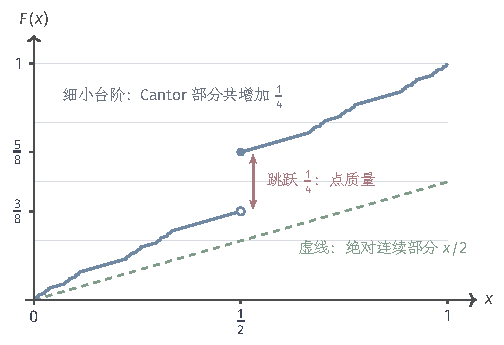
\includegraphics[width=85.425mm]{figures/02-abstract-mathematics/01-metric-and-measure/tikz/c4-increment-measure/figure.pdf}
  \caption{增量测度的三部分。蓝色曲线为$F(x)=x/2+\tfrac14\mathbf 1_{[1/2,1]}(x)+\tfrac14C(x)$，$C$为Cantor函数；绿色虚线$x/2$是绝对连续部分的累计，斜率$1/2$就是增量测度相对于长度的密度。$F$在$1/2$处从$3/8$跳到$5/8$（空心点为左极限，实心点为函数值），这$1/4$的增量是点质量；曲线上细小的台阶来自Cantor函数，它连续却在零长度的Cantor集上共增加$1/4$。曲线坐标在步长$1/243$的网格上计算。}
  \label{fig:density-increment}
\end{figure}

这个例子说明，“$F$连续”“$F$有界变差”“$F$几乎处处可导”都不足以保证增量测度有密度，必须要求绝对连续。把跳跃去掉后的$x/2+\tfrac14C(x)$已经连续，却仍有$\tfrac14$的奇异连续增量无法用密度表示。

\subsection{推前测度的密度}
\label{sec:density-pushforward}

随机变量经过一个函数变换后，分布变成推前测度（第~\ref{sec:measure-pushforward}节）。若输入测度有密度，输出测度是否有密度、怎样计算？第~\ref{sec:integral-change-of-variables}节已经建立了光滑换元公式，这里用它直接算出输出密度，不重复Jacobian公式的证明。

\paragraph{可逆光滑变换}
设$U,V\subseteq\mathbb R^d$是开集，$T:U\to V$是$C^1$微分同胚，即$T$可逆，且$T$与$T^{-1}$都连续可微。设$U$上的Borel测度$\mu$相对于$\lambda_d$有密度$p$。

\begin{theorem}[推前测度的密度]
\label{thm:density-pushforward}
在上述条件下，$T_\#\mu$相对于$V$上的$\lambda_d$有密度
\[
 q(\bm y)=p\bigl(T^{-1}(\bm y)\bigr)\,\bigl|\det DT^{-1}(\bm y)\bigr|,\qquad \bm y\in V .
\]
\end{theorem}

\begin{proof}
记$S=T^{-1}:V\to U$，它也是$C^1$微分同胚。把光滑换元公式（定理~\ref{thm:integral-jacobian-change}）用于$S$，对$U$上的非负可测函数$g$有
\[
 \int_Ug(\bm x)\,\mathrm d\bm x=\int_Vg\bigl(S(\bm y)\bigr)\,\bigl|\det DS(\bm y)\bigr|\,\mathrm d\bm y .
\]
对Borel集$B\subseteq V$，由推前测度的定义和密度的定义，
\[
 T_\#\mu(B)=\mu\bigl(T^{-1}(B)\bigr)=\int_U\mathbf 1_B\bigl(T(\bm x)\bigr)p(\bm x)\,\mathrm d\bm x .
\]
取$g(\bm x)=\mathbf 1_B(T(\bm x))p(\bm x)$，则$g(S(\bm y))=\mathbf 1_B(\bm y)p(S(\bm y))$，代入上式得
\[
 T_\#\mu(B)=\int_Bp\bigl(S(\bm y)\bigr)\,\bigl|\det DS(\bm y)\bigr|\,\mathrm d\bm y .
\]
\end{proof}

公式中的$|\det DT^{-1}(\bm y)|=1/|\det DT(T^{-1}(\bm y))|$度量了$T$在原像附近把体积压缩或拉伸的倍数：体积被拉伸的地方，同样多的质量摊到更大的范围，密度就变小。一维例子：$(0,1)$上的均匀概率$p=1$经$T(x)=-\ln x$映到$(0,+\infty)$，$T^{-1}(y)=\mathrm e^{-y}$，$|(T^{-1})'(y)|=\mathrm e^{-y}$，所以输出密度$q(y)=\mathrm e^{-y}$，即指数分布，$\int_0^\infty\mathrm e^{-y}\,\mathrm dy=1$。仿射变换$T(\bm x)=\bm A\bm x+\bm b$（$\bm A$可逆）给出$q(\bm y)=p(\bm A^{-1}(\bm y-\bm b))/|\det\bm A|$。

\paragraph{分支相加}
许多变换不是整体可逆的，例如$T(x)=x^2$把$x$与$-x$送到同一点。按第~\ref{sec:integral-change-of-variables}节分支换元的方式处理：设$U_1,U_2,\dots$是$U$中有限或可数个两两不交的开集，$U\setminus\bigcup_kU_k$是Lebesgue零测集，$T$在每个$U_k$上的限制$T_k:U_k\to V_k$是到开集$V_k$的$C^1$微分同胚，$S_k=T_k^{-1}$。因为$\mu\ll\lambda_d$，未纳入分支的部分也是$\mu$零测集。对Borel集$B$，
\[
 T_\#\mu(B)=\sum_k\mu\bigl(T^{-1}(B)\cap U_k\bigr)=\sum_k\int_{V_k}\mathbf 1_B(\bm y)\,p\bigl(S_k(\bm y)\bigr)\,\bigl|\det DS_k(\bm y)\bigr|\,\mathrm d\bm y,
\]
每一项用的是定理~\ref{thm:density-pushforward}的计算。被加项非负，由单调收敛定理可交换求和与积分，所以$T_\#\mu$的密度为
\[
 q(\bm y)=\sum_k\mathbf 1_{V_k}(\bm y)\,p\bigl(S_k(\bm y)\bigr)\,\bigl|\det DS_k(\bm y)\bigr| .
\]
各分支的像$V_k$可以重叠；在重叠处，所有原像分支的贡献都要累加。只取一个逆分支会遗漏质量。

\paragraph{平方变换}
取$[-1,1]$上的均匀概率测度，密度$p=1/2$，$T(x)=x^2$。两个分支是$U_1=(0,1)$与$U_2=(-1,0)$，未纳入的$\{-1,0,1\}$是零测集；两支的像都是$V_1=V_2=(0,1)$，逆映射$S_1(y)=\sqrt y$，$S_2(y)=-\sqrt y$，导数绝对值都是$1/(2\sqrt y)$。两支相加，
\[
 q(y)=\frac12\cdot\frac1{2\sqrt y}+\frac12\cdot\frac1{2\sqrt y}=\frac1{2\sqrt y},\qquad 0<y<1,
\]
在$(0,1)$外$q=0$。检查总质量：$\int_0^1\frac1{2\sqrt y}\,\mathrm dy=\bigl[\sqrt y\bigr]_0^1=1$。再核对一个集合：$B=[0.36,0.49]$的原像是$[-0.7,-0.6]\cup[0.6,0.7]$，输入质量为$0.2\times\tfrac12=0.1$；用输出密度计算，$\int_{0.36}^{0.49}\frac1{2\sqrt y}\,\mathrm dy=0.7-0.6=0.1$。若只取正分支，得到的$1/(4\sqrt y)$总积分只有$1/2$。

输出密度在$y\to0$时无界，但仍可积，所以原点附近的质量趋于零。原点的原像只有单点$\{0\}$，输入质量为$0$，故$T_\#\mu(\{0\})=0$，输出没有额外的点质量。若输入在$0$处有点质量，例如$\tfrac12\lambda|_{[-1,1]}$换成$\tfrac12\delta_0+\tfrac14\lambda|_{[-1,1]}$，推前后就会在$0$处出现点质量$\tfrac12$，这部分不能用相对于长度的密度表示。图~\ref{fig:density-square-branches}对照了输入端的两个原像区间与输出端的面积。

\begin{figure}[!htbp]
  \centering
  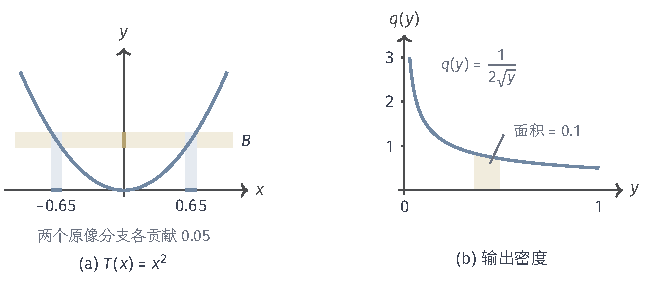
\includegraphics[width=110.144mm]{figures/02-abstract-mathematics/01-metric-and-measure/tikz/c4-square-branches/figure.pdf}
  \caption{平方变换下推前测度的密度。(a)$[-1,1]$上的均匀概率经$T(x)=x^2$映到$[0,1]$；输出区间$B=[0.36,0.49]$（黄色带）有两个原像分支$[-0.7,-0.6]$与$[0.6,0.7]$（蓝色条），各贡献质量$0.05$。(b)两支相加得到的输出密度$q(y)=1/(2\sqrt y)$，$B$上的面积为$0.1$，与输入端的质量一致；曲线在$y=1/36$处截断，$y\to0$时无界但可积。}
  \label{fig:density-square-branches}
\end{figure}

\section{本章小结}
\label{sec:density-summary}

本章从两个测度的比较出发，研究能否用一个逐点权重把参考测度换算成目标测度。第~\ref{chap:measures}章的绝对连续只说明零测集的包含关系；Radon–Nikodym定理表明，在两个测度都$\sigma$有限时，这个关系足以产生一个函数表示$\nu(A)=\int_Ah\,\mathrm d\mu$，并且该函数在$\mu$-几乎处处意义下唯一。证明的核心是在所有“不超过$\nu$”的候选权重中取积分最大者，再用Hahn分解说明剩余质量必为零。反过来，任何非负权重都能产生一个绝对连续的测度，这一方向不需要有限性条件。换测度公式把密度的作用从集合推广到函数，使目标测度下的积分化为参考测度下的加权积分。Lebesgue分解则保留了参考测度看不见的奇异质量：密度只表示绝对连续部分，点质量和Cantor测度这样的奇异连续质量都在密度之外。

使用密度时需要随时说明三件事。第一是参考测度：同一个目标测度相对于计数测度、几何权重或长度测度有不同的密度，不同参考下的密度不能直接相加，混合质量可以通过选择共同参考统一表示。第二是成立条件：存在性与唯一性需要$\sigma$有限，计数测度与长度的反例说明这一条件不能随意去掉；有符号测度要求总变差绝对连续，对应密度绝对可积；倒数公式只在测度等价时成立。第三是几乎处处：密度在参考零测集上的取值没有意义，链式规则与倒数公式都只在相应测度的几乎处处意义下成立。

离散质量、函数增量和映射后的质量是计算密度的三种常见入口。离散情形逐点相除；增量测度相对于长度的密度是导数，函数的绝对连续与测度的绝对连续在这里合而为一；推前测度的密度由Jacobian因子给出，多个分支的贡献需要累加。接下来的概率空间部分将在这些基础上继续：把一个随机量相对于较粗的信息作平均，需要在一个子$\sigma$代数上比较两种测度并取密度，条件期望正是这样定义的；比较两个概率分布的各种差异，也从它们相对于共同参考的密度出发。

